 \documentclass[12pt,english]{article}
\usepackage[utf8]{inputenc}
\markright{Weedop et al.\hfill The Effect of Phylogenetic Uncertainty and Imputation on EDGE Scores\hfill}
\usepackage{geometry}
\geometry{verbose,letterpaper,tmargin=2.54cm,bmargin=2.54cm,lmargin=2.54cm,rmargin=2.54cm}
%\geometry{verbose,letterpaper,tmargin=.1cm,bmargin=.1cm,lmargin=.1cm,rmargin=.1cm}
\usepackage{graphicx}
\DeclareGraphicsExtensions{.pdf,.png,.jpg}
\usepackage{amssymb,amsmath}
\usepackage{epstopdf}
\usepackage{tocbibind}
\usepackage[toc,page]{appendix}
\usepackage{supertabular}
\DeclareGraphicsRule{.tif}{png}{.png}{`convert #1 `dirname #1`/`basename #1 .tif`.png}
\usepackage{url}
\usepackage{subcaption}
\usepackage{caption}
\usepackage[super]{nth}
\usepackage{lineno} \linenumbers
\usepackage[doublespacing]{setspace}
\usepackage[parfill]{parskip}
\setlength{\parindent}{0pt}
\usepackage[citestyle=authoryear,bibstyle=authoryear,sorting=nyt,maxcitenames=2,maxbibnames=10,minbibnames=6,doi=false,url=false,isbn=false,firstinits=true,uniquename=false,uniquelist=false]{biblatex}
\bibliography{edge_sims}
\renewbibmacro*{name:andothers}{% Based on name:andothers from biblatex.def
  \ifboolexpr{
    test {\ifnumequal{\value{listcount}}{\value{liststop}}}
    and
    test \ifmorenames
  }
    {\ifnumgreater{\value{liststop}}{1}
       {\finalandcomma}
       {}%
     \andothersdelim\bibstring[]{andothers}}
    {}}
\renewcommand*{\finalnamedelim}{%
  \ifnumgreater{\value{liststop}}{2}{\finalandcomma}{}%
  \addspace\&\space}
\renewbibmacro{in:}{}
\AtEveryBibitem{%
  \clearfield{day}%
  \clearfield{month}%
  \clearfield{endday}%
  \clearfield{endmonth}%
}
\DeclareFieldFormat[article]{citetitle}{#1}
\DeclareFieldFormat[article]{title}{#1}
\DeclareFieldFormat[article]{pages}{#1}
\DeclareNameAlias{sortname}{last-first}

\usepackage{changes}
\setdeletedmarkup{\textcolor{red}{\sout{#1}}}

\begin{document}
\setlength{\parindent}{0pt}
\section*{Title page}

\textbf{Article title}: The Effect of Phylogenetic Uncertainty and Imputation on EDGE Scores

\textbf{Running head}: The Effect of Phylogenetic Uncertainty and Imputation on EDGE Scores

\textbf{Authors:} K.\ Bodie Weedop$^{1}$, Arne \O. Mooers$^2$, Caroline M.\ Tucker$^3$, and William D.\ Pearse$^{1}$\

$^1$ Department of Biology \& Ecology Center, Utah State University,
5305 Old Main Hill, Logan UT, 84322

$^2$ Department of Biological Sciences, Simon Fraser University, Burnaby,
British Columbia, Canada

$^3$ Department of Biology, University of North Carolina–Chapel Hill

$^*$To whom correspondence should be addressed:
\url{will.pearse@usu.edu}

\textbf{Word-count}: 5680 (abstract, main text, acknowledgments, and
  references)

\clearpage
\section*{Abstract}

Faced with saving as much diversity as possible under constraints, conservation
biologists can consider the contribution of a species to overall evolutionary
diversity. Metrics such as EDGE (Evolutionary Distinct and Globally Endangered)
have been successfully used to set conservation priorities for a number of taxa,
such as mammals, birds, corals, amphibians, and sharks. Each of these
applications of EDGE has required some form of correction for species whose
position within the tree of life are unknown. Perhaps the most advanced of these
corrections is phylogenetic imputation, but to date there has been no systematic
assessment of the impact of both missing species and imputation to correct for
them. Here we perform such a systematic assessment, simulating the random
missingness of species from a phylogeny, the imputation of the position of those
species, and measure the impact each of these processes has on the data
underlying EDGE scores. We find that EDGE ranking is remarkably robust to
missing species, and that phylogenetic imputation, while unbiased, is not
accurate in reconstructing species’ true evolutionary distinctiveness. On the
basis of these results, we provide clear guidance for EDGE scoring in the face
of phylogenetic uncertainty.

\textbf{Keywords}: conservation prioritization, evolutionary distinctiveness, 
EDGE, phylogenetic imputation.

\clearpage
\section*{Introduction}

Evidence from the fossil record and present-day studies argue we are in the
midst of, or entering, a sixth mass extinction \autocite{Barnosky2011,
Ceballos2015}, such that more populations than ever are declining and species
face heightened danger of extinction \autocite{Wake2008, Thomas2004}. Habitat
destruction \autocite{Brooks2002}, invasive species \autocite{Molnar2008},
climate change \autocite{Pounds2006}, and disease \autocite{Lips2006} are some
of the leading causes of species declines globally. Conservation biologists seek
to reduce these detrimental effects on species populations, but in reality they
have limited resources with which to do so. This challenge, termed the “Noah’s
Ark problem” \autocite{Weitzman1998}, has driven conservation biologists
identify different ways by which to prioritize, or triage, their resource
allocation \autocite{Bottrill2008}.

Conservation triage, like all sound decision-making, requires an index  with
which to quantify the relative urgency or importance for conservation among a
set of options. This allows scientists and policy-makers to use data to quantify
need and inform conservation decision-making and management activities. One such
triage strategy uses the EDGE metric to identify and prioritize species that are
Evolutionarily Distinct and Globally Endangered \autocite{Isaac2007}.
Evolutionary Distinctiveness (ED) measures the relative contributions to
phylogenetic diversity made by each species within a particular clade, assigning
each branch length equally to all the subtending species \autocite{Isaac2007},
Global Endangerment (GE), assigns numerical values to each of the World
Conservation Union (IUCN) Red List Categories. As species become increasingly
threatened and are placed into categories of increasing concern (\emph{e.g.}
from Vulnerable to Endangered), the GE numerical value increases. Species’ EDGE
score is intended to equally reflect a species’ evolutionary distinctiveness and
conservation status \autocite[even if it does not always in practice; see
][]{Pearse2015}.

Though originally used to prioritize global mammals, the EDGE metric has
subsequently been applied to a variety of taxonomic groups, including amphibians
\autocite{Isaac2012}, birds \autocite{Jetz2014}, corals \autocite{Curnick2015},
squamate reptiles \autocite{Tonini2016}, and sharks \autocite{Stein2018}.
Additional related metrics have also been developed, each emphasizing subtly
different things, such as the expected contribution of each species to future
phylogenetic diversity \autocite[HEDGE, I-HEDGE;][]{Steel2007,Jensen2016}, our
uncertainty over a species' future \autocite[EDAM;][]{Pearse2015}, and the
complementarity of a set of species \autocite{Faith2008}. The development and
expansion of EDGE-like metrics mirrors progress in other areas of conservation
biology, where the likelihood of success in conservation \autocite{Wilson2007,
Mcbride2007}, relative cost of certain interventions \autocite{Naidoo2006}, and
complementarity of interventions \autocite{Pressey1993, Myers2000} have received
attention. The EDGE index was developed explicitly with the intention of
informing conservation triage, and is now the basis of the global EDGE of
Existence Program (http://www.edgeofexistence.org/). The successful application
of EDGE in this program highlights the potential for phylogenetic conservation
prioritization metrics to provide actionable insights in the face of uncertainty
about species’ attributes. Nonetheless, almost every application of an EDGE-type
approach has to deal with the uncertainty resulting from missing data.

Missing data can affect confidence in EDGE scores in several ways. First, the
IUCN identifies some species as Data Deficient \autocite{Iucn2001, Iucn2008}.
which will affect the GE component of a species’ EDGE score. Fortunately, the
IUCN provides guidance for using any available contextual data to assign some
threat status to such species. A number of studies illustrate how to assign
threat categories to Data Deficient species, which in turn should reduce the
uncertainty in GE \autocite{Good2006, Butchart2010, Morais2013, Dulvy2014}. The
issue of missing phylogenetic data is arguably more complicated because here not
only does the focal species have no ED score, but ED scores of related species
that are on the tree can also be affected. Species of conservation concern are
almost by definition rare, and frequently lack sufficient DNA (or even
morphological) data to be placed with certainty on a phylogeny. For most
empirical EDGE lists, taxonomic information rather than sequence data alone is
used to place species in the tree of life \autocite[see]{Isaac2007, Isaac2012,
Collen2011, Jetz2014, Curnick2015, Stein2018, Gumbs2017}. Yet, to our knowledge,
there has yet to be a systematic study of the effect of such imputation on
species’ EDGE scores, unlike in other aspects of comparative biology
\autocite{Kuhn2011, Thomas2013}. Yet, to our knowledge, there has yet to be a
systematic study of the effect of such imputation on species' EDGE scores,
unlike in other aspects of comparative biology \autocite{Rabosky2014}. Indeed,
the fidelity of EDGE scores between imputed and non-imputed phylogenies and the
magnitude of error phylogenetic imputation introduces, are not known. As the
desire to use EDGE-type measures and phylogenies for conservation triage grows,
the need for consensus on how to resolve cases of phylogenetic uncertainty
becomes increasingly urgent.

Here we attempt to quantify the effect of missing species on EDGE rankings and
assess the degree to which imputation overcomes the effect of missing
phylogenetic data. We do so by simulating the removal of species from simulated
trees in two ways: at random and in a phylogenetically biased manner. By doing
so, we hope to provide two reasonably realistic case-studies of how species
might be expected to be missing from the tree of life. We then assess the extent
to which remaining species EDGE scores change, and we see how imputed species’
(species which have been removed and grafted back on) EDGE rankings correlate
with their true values. We simulate phylogenies, choose clades at random to
remove, and then impute the structure of these clades, all under the same model
of diversification. In so doing, we hope to provide clear guidance as to the
applicability of phylogenetic imputation as a solution for species missing
phylogenetic data. From our results, we argue that species’ ED values are
remarkably robust to missing species, but that phylogenetic imputation does not
reliably reconstruct the true ranking of those missing species.

\section*{Methods}

Here we use a simulation approach to test the effect of missing species (through
species removal from simulated phylogenies) and imputing species on a phylogeny
on species’ ED (Evolutionary Distinctiveness) scores. We focus exclusively on
the ED-component of the EDGE metric, since uncertainty in species GE scores has
already been addressed by the IUCN’s proposal to assign Data Deficient species
scores \autocite{Iucn2001, Iucn2008}. Because EDGE is the product of both ED and
GE components \autocite[see]{Isaac2007}, even perfectly accurate GE values could
be associated with imperfect EDGE scores if the ED scores are inaccurate .


All simulations and analyses were performed using R \autocite[version
3.4.0;][]{R2017}, and we performed 100 replicate simulations of each parameter
combination. All trees (both starting and imputed) were simulated under a
pure-birth Yule model using the sim.bdtree function under parameters of in the
\texttt{sim.bdtree} function under parameters of \texttt{(b=1, d=0)} in the
\texttt{geiger} R package \autocite{Pennell2014}. This particular model was
chosen because it is the simplest model possible: speciation rates are constant
across the entire tree of life and there is no extinction. We acknowledge that
more complex and/or biologically realistic models of diversification could
potentially improve the performance of imputation. However, we suggest that
imputation under a simple model that is identical to that used to simulate the
data is a low, and fair, benchmark for a method to meet. We used
\texttt{ed.calc} in the R package \texttt{caper} to calculate ED values
\autocite{Orme2013}. All our analysis code is available online in the
supplementary materials and at https://github.com/bweedop/edgeSims.


\subsection*{The impact of missing species on EDGE scores}
Our first set of simulations assess the impact of missing species data on the ED
scores of remaining species, considering data missing either in a random or
phylogenetically-biased fashion. We simulated phylogenies of different sizes
(number of taxa: 64, 128, 256, ..., 2048, 4096) and then removed constant
fractions of tips from the tree (0\%, 1\%, 2\%, ..., 19\%, ..., 99\%). To
simulate species data that is randomly missing with respect to the phylogenetic
structure, we used the sample function in R to select the relevant fraction of
species (rounded to the nearest whole number) without replacement. To remove
species in a phylogenetically-biased manner, we used
\textcite{Felsenstein2005}'s threshold model. First, we simulated a trait under
a constant rate Brownian-motion model ($\sigma$=0.5, starting root value = 1)
using the \texttt{sim.char} function in the \texttt{geiger} R package
\autocite{Pennell2014}. Species were then removed from the tree if their
simulated trait was in the upper quantile matching the fraction of species to be
removed. For example, if 10\% of trait values were removed from the tree. This
results in closely related species being removed more often than expected at
random.

To quantify the effect of these manipulations, we calculated the ED values of
species that are not removed from a tree both before and after other trees are
pruned tree. We then examined the correlation between these ED scores to measure
the effect of species’ removal on ED scores. If missing species do not affect ED
values, we expect a strong, positive correlation between the ED scores
calculated before and after species were removed from the phylogeny. Note that
species removed from the phylogeny are omitted from this comparison. We outline
our approach in figure \ref{missingSpecies}.

\begin{figure}[!ht]
  \center
  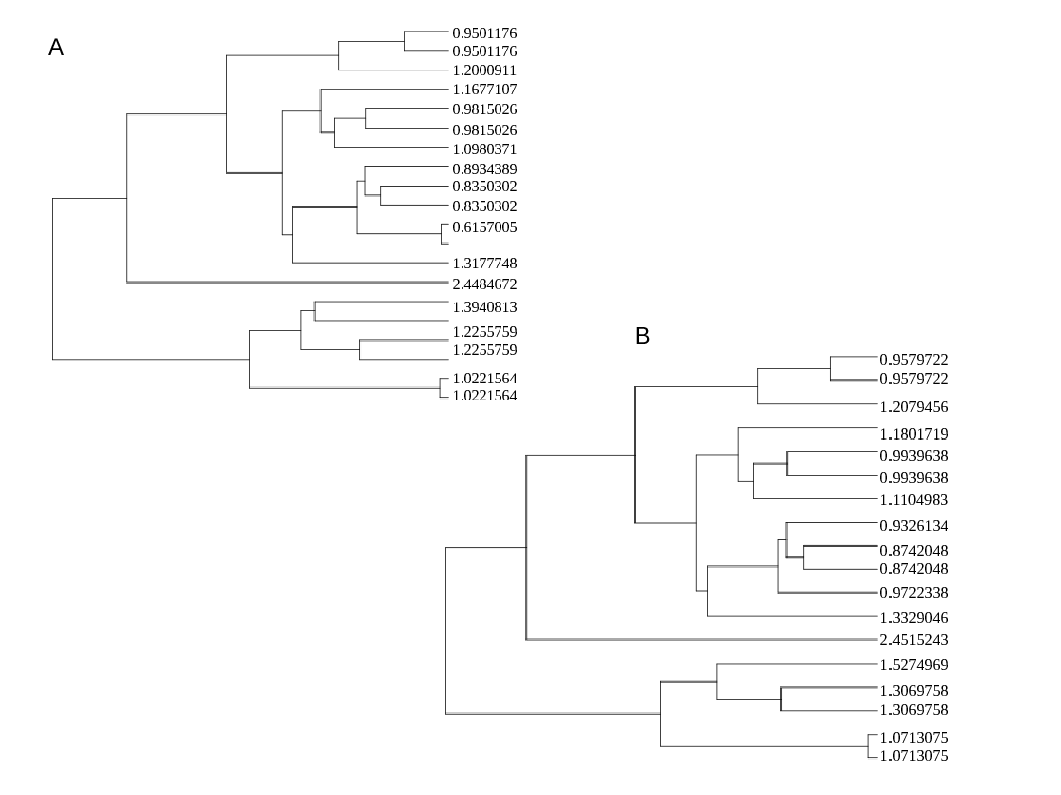
\includegraphics[width=.75\textwidth]{missingSpecies.png}
  \caption{\textbf{Example of simulated phylogenies and ED values used to
  compare species ED values.} The simulated tree on the left is the true tree
  prior to removal of missing species. On the right, is the same tree after
  missing species have been removed. We correlate the remaining ED values to
  compare the ED values. Dashed lines can be seen for the species which would
  have ED scores compared.}
  \label{missingSpecies}
\end{figure}

\subsection*{The impact of phylogenetic imputation on EDGE scores}
Our second set of simulations tested the impact of imputation on ED scores
within an imputed clade. We used relatively small clades (5, 6, 7, ..., 30, 31,
32 species) from phylogenies of different sizes (128, 147, 168, ... 776, 891,
1024 species). We first randomly selected a clade to be removed from the ‘true’
tree and then simulated a new phylogeny of the same size as the removed clade.
This newly simulated clade had the same pure-birth model used to generate the
original phylogeny. We then placed the newly simulated clade in the full
phylogeny, in the same location as the removed clade. If a newly simulated clade
was so old that it was not possible to graft it into place, we discarded that
clade and simulated another. Thus, we imputed each missing clade using the same
model used to generate it from the original tree: in an empirical study this
model would also have to be inferred, an additional source of error not
considered here. An overview of our approach is given in \ref{imputeConcept}. 

To assess whether clades, once imputed, had similar ED scores, we correlated the
imputed ED scores against true ED scores. We also calculated the sum of the
absolute change in ranked ED for each species, which is particularly relevant
for EDGE-listing as it is often the top 100, 200, etc., species on which
conservation actions are targeted. We modeled both of these metrics (the change
in ranking and the correlation) as a function of a number of potential
explanatory variables. Specifically, the estimated speciation rate of the
original phylogeny \autocite[using \texttt{ape::yule};][]{Paradis2004}, the sum
of all phylogenetic branch-lengths in the original phylogeny \autocite[Faith's
PD;][]{Faith1992}, the sum of all phylogenetic branch-lengths in the original
focal clade \autocite[Faith's PD;][]{Faith1992}, the value of gamma in the
original phylogeny \autocite[using \texttt{phytools::gammatest}][]{Pybus2000,
Revell2012}, colless’ index of the original phylogeny
\autocite[using\texttt{apTreeshape::as.treeshape};][]{Colless1982,
Bortolussi2009}, the kurtosis of species’ ED values in the original phylogeny
\autocite[using \texttt{moments::kurtosis};][]{Komsta2015}, the skew of species’
ED values in the original phylogeny \autocite[using
\texttt{moments::skew};][]{Komsta2015}, the total number of species in the
original phylogeny, and the total number of species within the imputed clade.
Although the expectations of many of these explanatory variables are known for
Yule trees, in each simulation they are expected to vary somewhat by chance.

Across the clades within a phylogeny, each clade possesses an expected ED value
(\emph{i.e.} an average ED score). This value can be calculated for clades which
possess missing species and assigned to such species in order to include them in
the overall ranking. A version of this method has been performed in the past to
produce EDGE rankings for tetrapods \autocite{Gumbs2017}. To test this method,
we assigned the average ED of the selected clade to each of its' species and
compared the ranking of the average ED value to the rank of the true ED value.
We calculated the sum of the absolute change in the ranked ED for each species
within the selected clade.

\begin{figure}[!ht]
  \center
  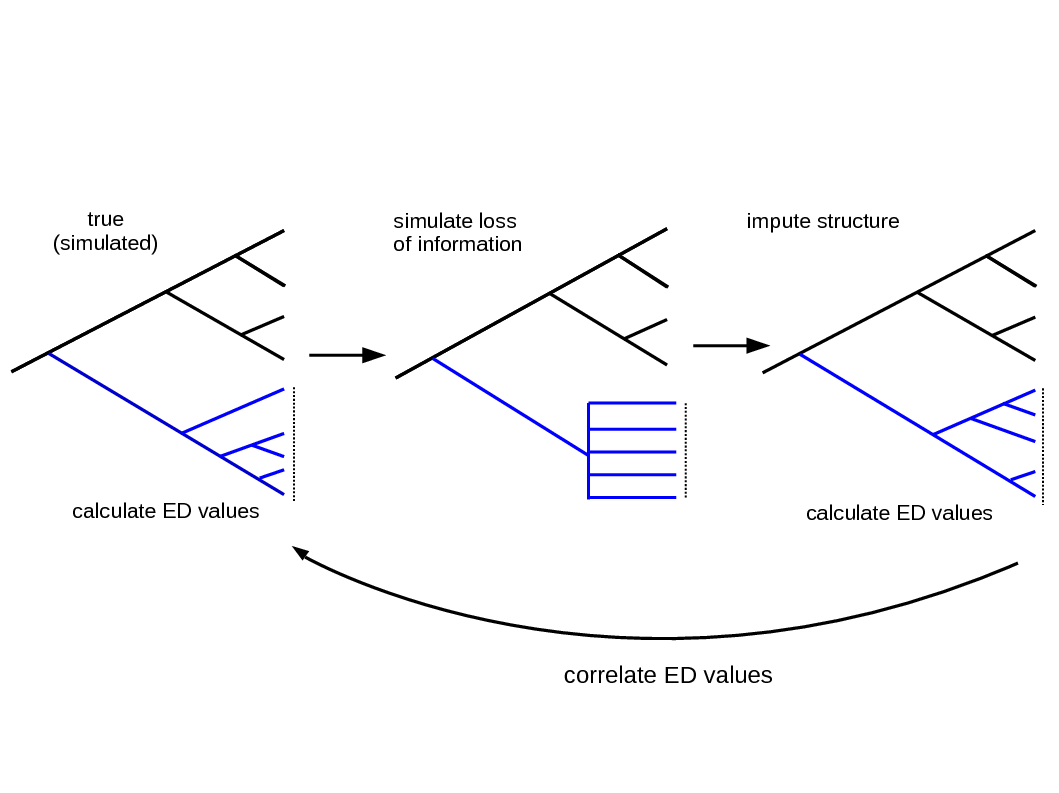
\includegraphics[width=.75\textwidth]{imputeConcept.png}
  \caption{\textbf{Conceptual overview of the simulations conducted in this
  study.} In (a), the simulated tree on the left is the ‘true tree’ prior to
  removal of missing species. On the right is the same tree after the removal of
  missing species. We calculated ED values for both the true tree and the
  incomplete tree, and calculated the correlation between ED values for species
  common between these trees (indicated with dashed lines) to measure the impact
  of missing species on known species’ scores. In (b), the simulated tree on the
  left is the ‘true tree’. We selected a clade to treat as ‘missing’
  (highlighted with a dashed line) by replacing it with a polytomy (middle
  panel) , and then imputed the ‘missing’ species following the procedure
  described in the Methods to produce the imputed clade (dashed line) in the
  right panel. To compare true and imputed ED values within the imputed clade,
  we correlated ED values calculated on the true clade with those for the
  imputed clade. }
  \label{imputeConcept}
\end{figure}

\section*{Results}
When species data was missing (\emph{i.e.} dropped from the phylogeny) under
both random and phylogenetically-patterned loss, species’ ED scores are slightly
less accurate, particularly as the number of species missing increases (Table 1;
figure \ref{randomVsClustered}). ED values were less robust to
phylogenetically-biased missing species, as compared to those that are randomly
missing from the tree. If 20\% of species are missing, the average correlation
between true and estimated ED is 0.88 and 0.94 for phylogenetically-biased and
random missing species, respectively.

\begin{figure}[!ht]
  \center
  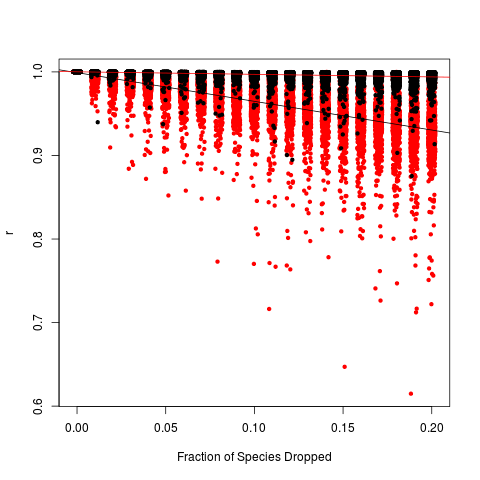
\includegraphics[width=.5\textwidth]{randomVsCluster.png}
  \caption{\textbf{Correlation coefficient values plotted against the fraction
  of species dropped, either at random or in a clustered manner.} The color of
  data points denote whether species were missing from the phylogeny at randomly
  (orange; n = 100) or in clustered manner (grey; n = 100). Lines show the
  relationship between correlation coefficients when species are dropped at
  random (red), or in a clustered manner (black). Correlations are calculated
  for the the ED values before and after species are dropped from the phylogeny.
  }
  \label{randomVsClustered}
\end{figure}

\begin{table}[ht]
  \centering
  \begin{tabular}{rrrrr}
    \hline
      & Estimate & Std. Error & t value & Pr($>$$|$t$|$) \\
      \hline
      (Intercept) & 1.0315 & 0.0013 & 821.39 & $<$0.0001 \\
      Fraction of Species Dropped & -0.4696 & 0.0020 & -233.16 & $<$0.0001 \\
      Random Treatment & 0.0630 & 0.0018 & 35.47 & $<$0.0001 \\
      Number of Species Overall & 0.0000 & 0.0000 & 7.89 & $<$0.0001 \\
      Fraction of Species Dropped:Random Treatment & -0.2774 & 0.0028 & -97.45 & $<$0.0001 \\
      Random Treatment:Number of Species Overall & 0.0000 & 0.0000 & -4.38 & $<$0.0001 \\
      \hline
    \hline
  \end{tabular}
\caption*{\textbf{Table 1: ANCOVA model summary describing the effect of
dropping species on remaining species ED Values.} The fraction of species
missing significantly affects the remaining ED values. Species missing at
random and in a clustered manner both have negative effects on the ED values of
species remaining on the tree ($F_{139696, 5}$ = 40350, $R^{2}$ = 0.5908,
p$<$0.0001).}
\end{table}

When clades were imputed on the tree, we found no average positive correlation
between the imputed ED and true ED values for species within the imputed clades
(figure \ref{imputationTrend}, table 2). The mean or expected correlation was 0.
We also found no explanatory variables that explained significant variation in
this relationship (table 2; see also Supplementary Materials). However, we did
find evidence that, when imputing larger clades, the variation in the
correlation between true and imputed ED scores decreases, although it remains
centered around zero (see Supplementary Materials). When considering rankings
rather than raw scores, we similarly found large effects of imputation for the
imputed species (figure \ref{rankingError} and table 4). This ranking error
increased with the size of the imputed clade and phylogeny (table 4), and can
affect ranking error within the top 100 and 250 species (see Supplementary
Materials). To give an example of the magnitude of the effect, within a
phylogeny of 1024 species, the members of an imputed clade of 30 species are, on
average, $\pm$ 315 rankings from their true rankings.

Additionally, we found similar effects in ranking error when using the average
ED value of clade for a missing species (see Supplementary Materials). Also,
this ranking error increased with the size of the clade. For some context,
within a phylogeny of 1024 species, the members of an imputed clade of 30
species are, on average, $\pm$ 229 rankings from their true rankings. 


\begin{figure}[!ht]
  \center
  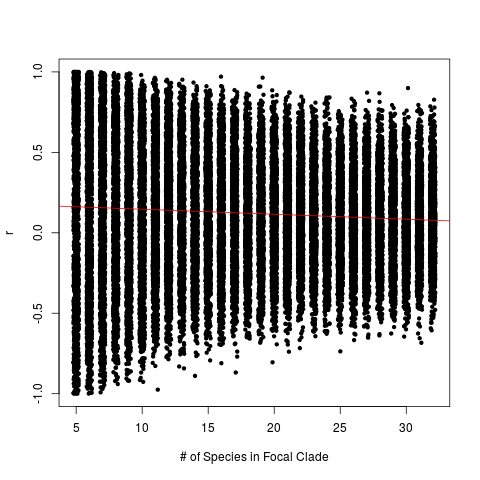
\includegraphics[width=.5\textwidth]{edModel.png}
  \caption{\textbf{Correlation coefficient-values plotted against the number of
  species in the focal clade.} Each data point  represents the correlation
  between ED values within the focal clades where imputation has occurred,
  comparing ED values for the true position of species with those calculated via
  the imputed tree. The regression line (red) and trend even closer to zero
  demonstrates the decrease in informative value of the imputed ED values. This
  is reinforced by the visual narrowing of r-values around zero.}
  \label{imputationTrend}
\end{figure}

\begin{table}[ht] 
\centering
\begin{tabular}{rrrrr}
  \hline
  & Estimate & Std. Error & t value & Pr($>$$|$t$|$) \\
   \hline
   (Intercept) & 0.1974 & 0.0501 & 3.94 & 0.0001 \\
   Size of Focal Clade & -0.0036 & 0.0005 & -7.60 & 0.0000 \\
   Size of Phylogeny & 0.0001 & 0.0001 & 0.60 & 0.5497 \\
   PD & -0.0001 & 0.0001 & -0.64 & 0.5241 \\
   Lambda & -0.0199 & 0.0493 & -0.40 & 0.6865 \\
   Colless' Index & -0.0000 & 0.0000 & -0.08 & 0.9380 \\
   Skew & 0.0022 & 0.0083 & 0.27 & 0.7885 \\
   Kurtosis & -0.0001 & 0.0008 & -0.16 & 0.8736 \\
   Depth of Imputed Clade & 0.0006 & 0.0005 & 1.27 & 0.2045 \\
   \hline
   \hline
\end{tabular}
\caption*{\textbf{Table 2: Effect of Clade Size on Imputed ED Values.} The
correlation between the true and imputed values is quite low, as shown by the
intercept, and declines further as the imputed clade size increases, this
correlation further decreases. The remaining variables are not significant
($F_{44791, 8}$ = 29.1, $R^{2}$ = 0.005, p$<$0.0001).}
\end{table}

\begin{figure}[!ht]
  \center
  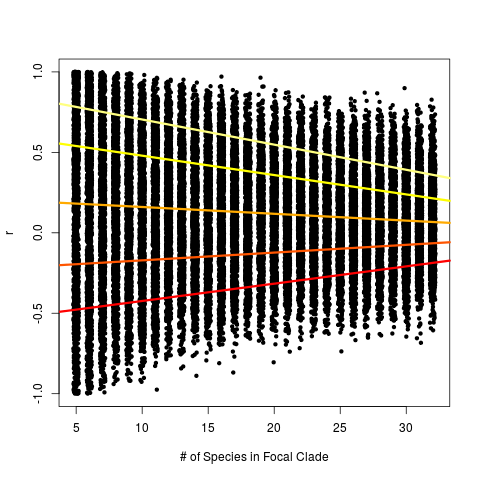
\includegraphics[width=.5\textwidth]{quantModel.png}
  \caption{\textbf{Quantile regression of r-values against size of imputed
  clades.} Each data point denotes a correlative comparison between ED values
  within the focal clades where imputation has occurred. Each regression line
  (top to bottom) represent quantile regressions from highest to lowest,
  respectively. Each of the regression lines demonstrate a convergence of the
  variation in r-values around zero.}
  \label{quantReg}
\end{figure}

\begin{table}[ht]
  \centering
  \begin{tabular}{rrrrrr}
    \hline
    & $\tau$ = 0.10 & $\tau$ = 0.25 & $\tau$ = 0.50 & $\tau$ = 0.75 & $\tau$ = 0.90 \\
    \hline
  (Intercept) & -0.53 & -0.22 & 0.20 & 0.60 & 0.86 \\
    Size of Focal Clade & 0.01 & 0.00 & -0.00 & -0.01 & -0.02 \\
    \hline
    \hline
  \end{tabular}
  \caption*{\textbf{Table 3: Quantile Regression of Clade Size and Total Species
  on Ranking Error.} Quantile regression model demonstrating the effect of clade
  size on the correlation between true and imputed ED values. The quantile
  regression estimates demonstrate statistical significance that as imputed
  clade size increases, variation in coefficient of correlation (r) between ED
  values center around zero (all p-values are $<$0.0001).}
\end{table}


\begin{figure}[!ht]
  \center
  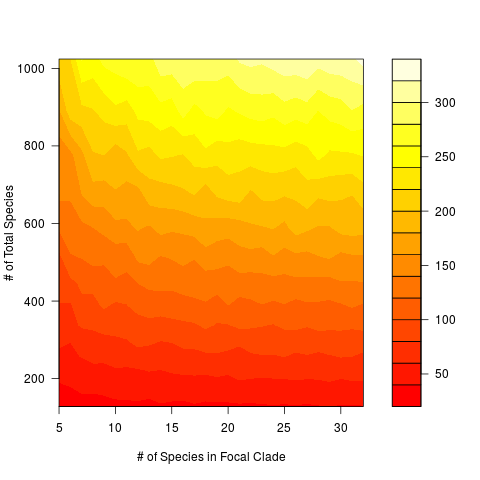
\includegraphics[width=.5\textwidth]{rankingError.png}
  \caption{\textbf{Mean ranking error of species within the focal clade.} The 
  gradient on the right demonstrates average number of positions within the 
  full ranking that focal clade species shifted from their true rank.
  While controlling for the size of the full phylogeny and focal clade, species 
  within the focal clade were, on average, ranked far from the true rank. }
  \label{rankingError}
\end{figure}

\begin{table}[ht]
  \centering
  \begin{tabular}{rrrrr}
    \hline
   & Estimate & Std. Error & t value & Pr($>$$|$t$|$) \\
    \hline
  (Intercept) & -1.6344 & 0.0332 & -49.29 & 0.0001 \\
    Size of Focal Clade & 0.0900 & 0.0010 & 91.22 & 0.0001 \\
    Size of Phylogeny & 0.5179 & 0.0013 & 383.99 & 0.0001 \\
     \hline
     \hline
  \end{tabular}
  \caption*{\textbf{Table 4: Effect of Clade Size and Total Phylogeny Size on
  Ranking Error.} Model demonstrating the relationship between focal clade
  species ranking error and the size of imputed clade and overall phylogeny.
  Square-root transformations have been applied to both ranking error and size
  of phylogeny. Significant increases in ranking error are seen when the sizes
  of both the imputed clade and the full phylogeny increase ($F_{47997, 2}$ =
  77890, $R^{2}$ = 0.7644, p$<$0.0001).}
  \end{table}

\clearpage
\section*{Discussion}
Phylogenies are increasingly advocated for conservation prioritization,
decision-making, and policy \autocite{Vezquez1998}. A major obstacle to a more
widespread adoption of phylogenetic prioritization methods such as EDGE is
phylogenetic uncertainty \autocite{Collen2015}. There is tension between the
need to make decisions to preserve biodiversity - including evolutionary history
- now, and the reality that we do not have complete information about the
phylogenetic placement of many species of conservation concern. The intention of
our study is to provide concrete information about the impact of such
phylogenetic uncertainty on conservation prioritization. To address this
uncertainty, we answered two key questions: (1) the extent to which species that
are missing from the tree of life impact the ED scores of species for which we
do have data, and (2) the extent to which phylogenetic imputation can accurately
fill in ED scores for taxa with no phylogenetic data. To the first question (1),
we found that while missing species do impact the ED scores of other species,
the effects are not always severe, particularly if species are missing at random
from the tree of life. For the second question (2), we found limited evidence
that phylogenetic imputation can reconstruct species’ ED scores and rankings.

Our results are derived solely from simulations under a simple model of
diversification — the Yule model. We do acknowledge that, in reality, lineages
evolve in more complex ways than are captured by such a simple model. However,
such complexities are unlikely to make imputation easier (in fact, they would
likely make imputation more difficult). We suggest that focusing on the simplest
model of diversification makes our results more generalizable. Further, we focus
here solely on the results from a single imputation in each simulation, despite,
empirically, biologists reporting average ED scores calculated across
pseudo-posterior distributions of many imputed phylogenies \autocite{Kuhn2011}.
Thus our simulations show that these averages are conducted across phylogenies
with large degrees of uncertainty. It is well-known that such methods are not
biased \autocite[indeed, this was originally shown by][]{Kuhn2011}: here we
emphasize that the uncertainty they introduce is sufficiently large that they
may be less informative than previously been thought.

\subsection*{ED scores are relatively robust to missing species}
Missing species and poor phylogenetic resolution have been identified as causes
of uncertainty when calculating ED \autocite{Isaac2007}, but we were unable to
find a quantitative assessment of how missing species might affect ED values of
species which are not missing. Empirically in corals, incomplete phylogenies
produced similar results as later, more complete trees \autocite{Curnick2015}.
Our results support this finding. Indeed, our analysis suggests that, on average
(and we emphasize that there is a good amount of variation about that average;
see \ref{randomVsClustered}), a phylogeny missing 20\% of species at random will
still have ED scores that are strongly correlated ($r$=0.94) with the true ED
scores.

We did find that missing species are more problematic when those species are
non-randomly distributed across the phylogeny. Our simulations do not cover
extreme phylogenetic patterning, such as if an entire clade were missing; this
is notable because clades that are geographically restricted to
difficult-to-reach regions are both difficult to sequence and not uncommon
\autocite[\added{as is seen with 27 coral species in the Indian
Ocean;}][]{Arrigoni2012}. Thus these results are likely conservative. We also do
not attempt to comprehensively simulate all of the different ways in which
species could be missing from a phylogeny. We simply demonstrate that, compared
to a scenario in which species are missing at random for which impacts are low,
the impacts of missing species can increase in non-random situations, such as if
the missing species are distributed across the phylogeny in a biased fashion.

\subsection*{Imputation does not reconstruct the ED value of species with great precision}
Our results show that imputation does not accurately recover the true ED values
nor the true ED rank of missing species (figure \ref{imputationTrend}; figure
\ref{rankingError}). Thus we argue that, even though under imputation, missing
species are incorporated into EDGE lists, their associated EDGE scores may not
accurately reflect their true scores. For example, members of an imputed clade
of 25 species within a phylogeny of 850 species are, on average, imputed to have
ED scores 250 ranks away from their true rank (figure \ref{imputationTrend}; Table
4). We acknowledge these are averages and may change depending on particular
phylogeny, but we can find no statistically significant predictors of that
variation.

While we did not assess clades with fewer than five species (we do not consider
correlations or averages to be reliable with so few data-points), we cannot
think why smaller clades would necessarily be more reliable (and this would be a
reversal of the trend in figure \ref{imputationTrend}). Indeed, in the smallest
possible clade (two species), imputation is essentially sampling a terminal
branch length from an exponential distribution \autocite{Kuhn2011}; such a
process should still lead to a great degree of uncertainty. Further, smaller
sample sizes should not lead to a more accurate estimate. It is, perhaps,
unsurprising that imputed ED values do not correlate with their true values (see
figure\ref{quantReg}), but we were surprised at the degree of ranking error.
Indeed, large phylogenies showed \emph{greater} ranking error; we na\"{i}vely
would have expected the opposite. We would have expected our upper bound on the
age of the imputed clade, which we would have expected to be relatively younger
in larger phylogenies, to have somewhat controlled the range of the ranks of our
imputed species. ED is known to be driven mostly by terminal branch length
\autocite{Redding2008, Isaac2007, Steel2007}; our results therefore emphasize
this.

Imputation is not the only way to incorporate missing species into EDGE-like
frameworks \autocite{Gumbs2017, Collen2011}, but it is likely the most common.
$3,330$ of birds \autocite[\textasciitilde30\%;][]{Jetz2014}, 250 of mammals
\autocite[\textasciitilde 5.6\%;][]{Collen2011}, and 610 of sharks
\autocite[\textasciitilde49\%;][]{Stein2018} in recent EDGE lists were imputed.
It is well-known that phylogenetic imputation can cause biases in other
statistical methods, such as the estimation of evolutionary phylogenetic signal
\autocite{Rabosky2014}. We emphasize that we are not suggesting that imputation
\emph{biases} ED scores: we are, instead, suggesting that it is less precise
than has previously been acknowledged. This result suggests that guidelines
might be useful.

\subsection*{Guidelines for the use of imputation}
The impact of imputation on EDGE scores is almost certainly less than its impact
on ED scores, because EDGE scores are a product of both ED and IUCN status
(‘GE’). However, the goal of EDGE-like measures is to incorporate phylogeny, and
if imputed EDGE scores are driven by their GE component because of uncertainty
introduced by imputation, this essentially creates another metric of IUCN
status.

Our results suggest that incomplete phylogenies can be used to estimate ED
scores with remarkably high degrees of accuracy. Instead of using imputation to
account for the relatively minor impact of missing species, we suggest
conservation biologists should focus on accounting for phylogenetic uncertainty
in the species for which they have data. While we have not explored this
uncertainty here, evolutionary biologists commonly work with distributions of
trees generated from genetic data \autocite[reviewed in][]{Huelsenbeck2001,
Bollback2005}, since the precise topology and dating of a phylogeny is almost
always uncertain. This uncertainty has, indeed, already been shown to affect
EDGE scores and rankings \autocite{Pearse2015}. We suggest conservation
biologists should focus on averaging across phylogenetic uncertainty as a
priority. There is, of course, nothing stopping biologists from also using
taxonomy to impute the positions of missing species within the phylogeny: being
thorough is a virtue, but it is important to focus on the major sources of
potential error first.

Our results suggest, strongly, that prioritizing species whose phylogenetic
structure has been imputed should be done with extreme care, if it at all. In
the case that an imputed species is imputed to be below a threshold set for
conservation (most EDGE studies focus on the ‘top 100’ species or something
similar), then the path forward is clear: that species should not have
conservation funds allocated to it at this time. The case where a species, on
average, is above a threshold is more complex, but the theory underlying
imputation can give some guidance. Imputed distributions of trees essentially
represent Bayesian posterior distributions \autocite{Kuhn2011}, and
so the 95\% posterior densities of these distributions’ ED values represent a
range within which we can be 95\% certain the true ED scores lie (if the model
assumptions are met). Thus we suggest that conservation action should only be
initiated for a species if there is a 95\% (or 80\%, or whatever confidence is
deemed appropriate) probability that it is above that threshold. Thus a species
whose 95\% ranking was 30–300 could not, with confidence, be called a top-100
species. Our results suggest that, on average, very few imputed species will
meet such a criterion.

Ultimately, we are currently fighting a losing battle to preserve the tree of
life. Our results are good news: they suggest that we can start right away using
the phylogenies we already have in-hand. The effect of missing species is mild
enough that we often do not need costly and time-consuming imputation, and
imputation rarely gives us sufficiently precise estimates of species’ ED scores
anyway. We suggest that, given we do not have the resources to save everything,
we should consider focusing our efforts on those species whose ED scores we can
know with greater certainty: those for which we have data.

\section*{Acknowledgments}
We are grateful to E.\ Simpson, M.\ Sneddon, J.\ Stachewicz, and XXX
anonymous reviewers for providing constructive feedback on this
manuscript.

\clearpage
\printbibliography

\clearpage
\appendix
\section*{A. Effect of Measures of the True, Full Phylogenies}

\begin{figure}[!ht]
  \center
  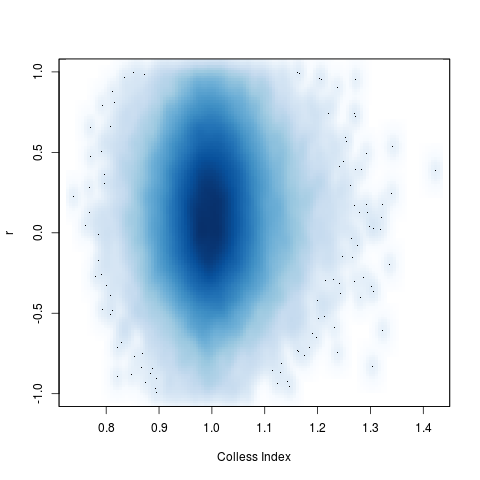
\includegraphics[width=.5\textwidth]{trueColless.png}
  \caption{\textbf{Effect of the True Colless Index of FullPhylogeny.}}
\end{figure}

\begin{figure}[!ht]
  \center
  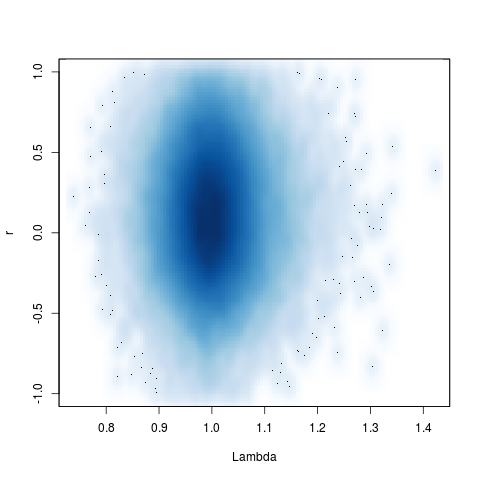
\includegraphics[width=.5\textwidth]{trueLambda.png}
  \caption{\textbf{Effect of the True Lambda of Full Phylogeny.}}
\end{figure}

\begin{figure}[!ht]
  \center
  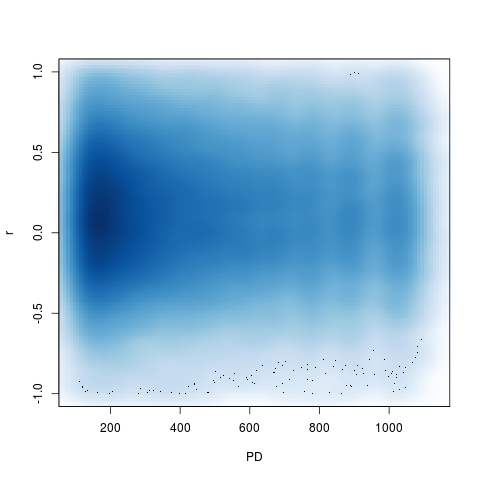
\includegraphics[width=.5\textwidth]{PD.png}
  \caption{\textbf{Effect of True PD of Full Phylogeny.}}
\end{figure}

\begin{figure}[!ht]
  \center
  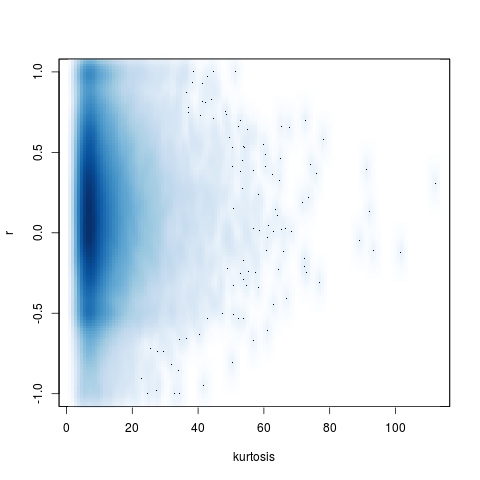
\includegraphics[width=.5\textwidth]{originalKurtosis.png}
  \caption{\textbf{Effect of the True Kurtosis of Full Phylogeny.}}
\end{figure}

\begin{figure}[!ht]
  \center
  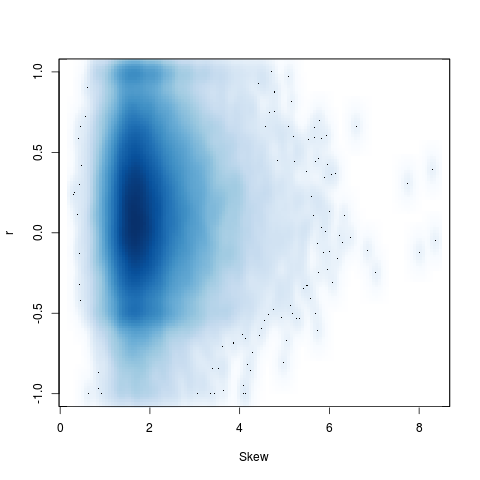
\includegraphics[width=.5\textwidth]{originalSkew.png}
  \caption{\textbf{Effect of the True Skew of Full Phylogeny.}}
\end{figure}

\begin{figure}[!ht]
  \center
  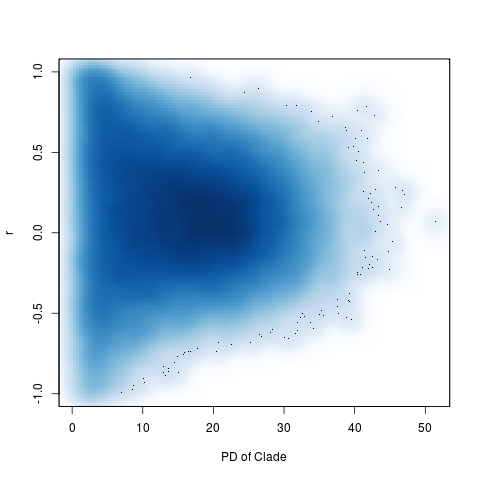
\includegraphics[width=.5\textwidth]{cladePD.png}
  \caption{\textbf{Effect of the True PD of The Selected Clade.}}
\end{figure}

\clearpage
\clearpage
\section*{B. Error Rate in Top Rankings}

\begin{figure}[!ht]
  \center
  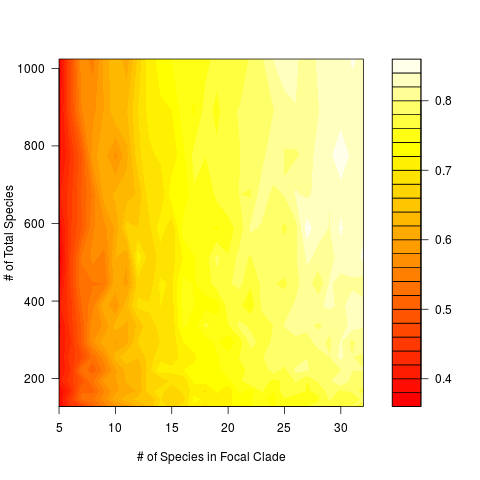
\includegraphics[width=.5\textwidth]{errorRate50.png}
  \caption{\textbf{Mean error rate in the ranking of top 50 species.}}
\end{figure}

\begin{figure}[!ht]
  \center
  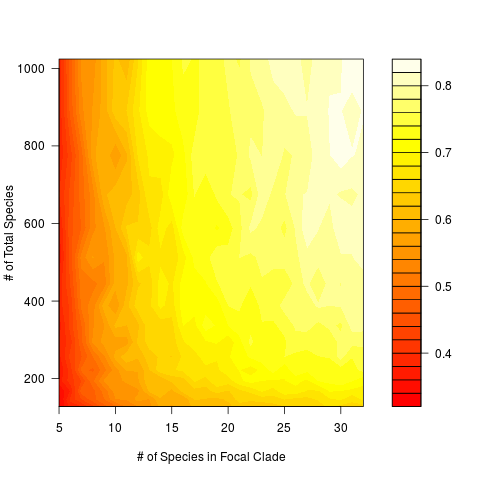
\includegraphics[width=.5\textwidth]{errorRate100.png}
  \caption{\textbf{Mean error rate in the ranking of top 100 species.} }
\end{figure}

\begin{figure}[!ht]
  \center
  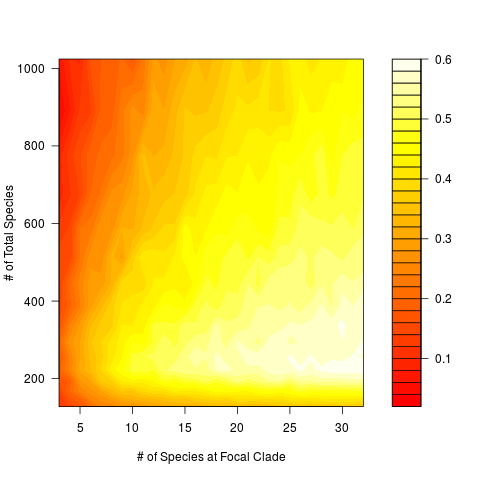
\includegraphics[width=.5\textwidth]{errorRate200.png}
  \caption{\textbf{Mean error rate in the ranking of top 200 species.} }
\end{figure}

\begin{figure}[!ht]
  \center
  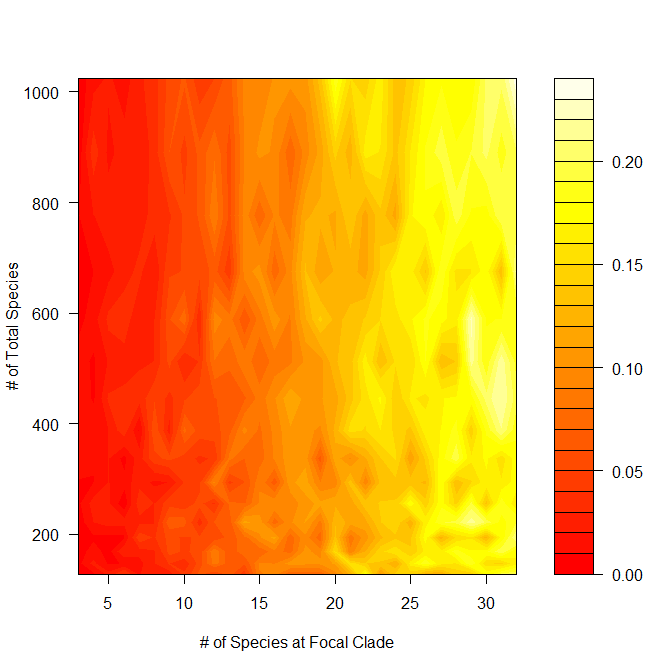
\includegraphics[width=.5\textwidth]{errorRate5pct.png}
  \caption{\textbf{Mean error rate in the ranking of top 5\% of species.} }
\end{figure}

\begin{figure}[!ht]
  \center
  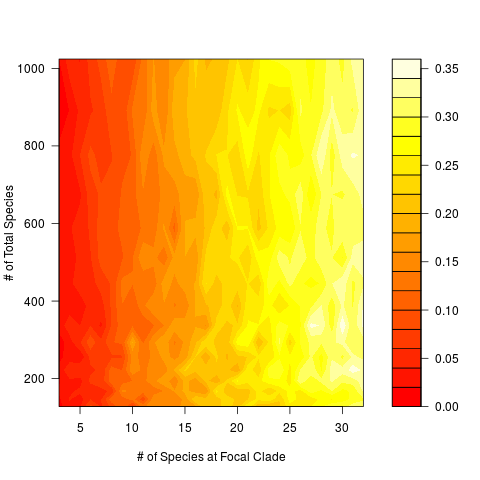
\includegraphics[width=.5\textwidth]{errorRate10pct.png}
  \caption{\textbf{Mean error rate in the ranking of top 10\% of species.} }
\end{figure}

\begin{figure}[!ht]
  \center
  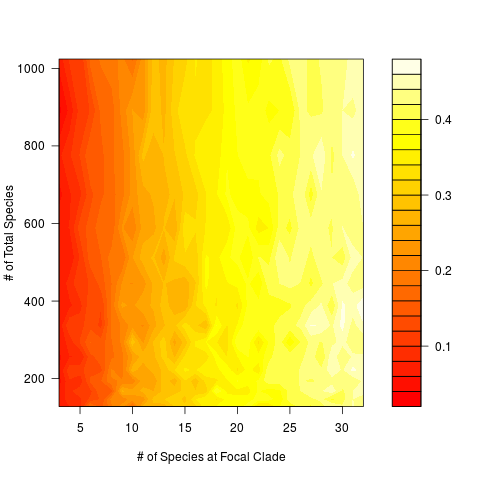
\includegraphics[width=.5\textwidth]{errorRate20pct.png}
  \caption{\textbf{Mean error rate in the ranking of top 20\% of species.}}
\end{figure}

\section*{C. Ranking Error When Using Average ED Value}

\begin{figure}[!ht]
  \center
  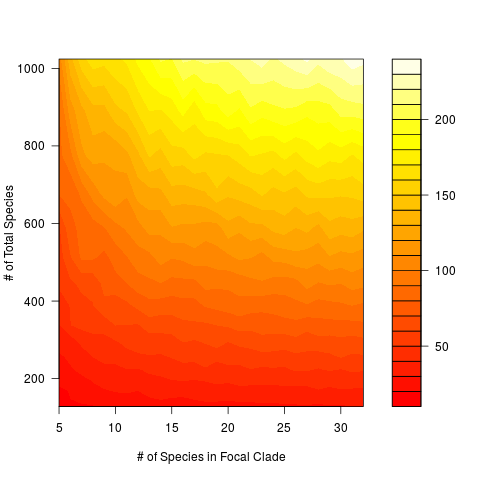
\includegraphics[width=.5\textwidth]{rankingError_avgEDforClade.png}
  \caption{\textbf{Mean Ranking Error of Species Assigned Average ED.} }
\end{figure}

\section*{D. Ranking Error of Non-imputed Species}

\begin{figure}[!ht]
  \center
  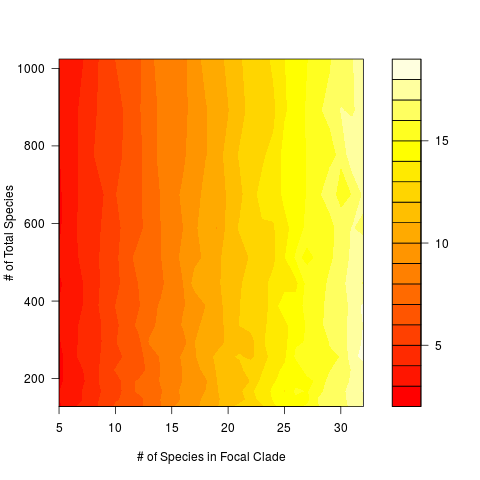
\includegraphics[width=.5\textwidth]{rankingError_remainingSpp.png}
  \caption{\textbf{Ranking Error of Non-imputed Species.} }
\end{figure}

\end{document}
%%% Local Variables:
%%% mode: latex
%%% TeX-master: t
%%% End:
